
\documentclass[10pt,twocolumn,letterpaper]{article}

\usepackage{iccv}
\usepackage{times}
\usepackage{epsfig}
\usepackage{graphicx}
\usepackage{amsmath}
\usepackage{amssymb}
\usepackage[numbers,sort]{natbib}

\usepackage{subfigure}
\usepackage{upgreek}
\usepackage{multirow}
\usepackage{color}
\usepackage{bm}
\DeclareMathOperator*{\argmin}{arg\,min}
\usepackage{arydshln}
\usepackage{latexsym}

\usepackage{amsthm}
\newtheorem{theorem}{Theorem}
\newtheorem{lemma}[theorem]{Lemma}
\newtheorem{conj}[theorem]{Conjecture}


% Include other packages here, before hyperref.

% If you comment hyperref and then uncomment it, you should delete
% egpaper.aux before re-running latex.  (Or just hit 'q' on the first latex
% run, let it finish, and you should be clear).
\usepackage[pagebackref=true,breaklinks=true,letterpaper=true,colorlinks,bookmarks=false]{hyperref}

% \iccvfinalcopy % *** Uncomment this line for the final submission

\def\iccvPaperID{572} % *** Enter the ICCV Paper ID here
\def\httilde{\mbox{\tt\raisebox{-.5ex}{\symbol{126}}}}

% Pages are numbered in submission mode, and unnumbered in camera-ready
\ificcvfinal\pagestyle{empty}\fi
\begin{document}

%%%%%%%%% TITLE
\title{Multi-channel weighted nuclear norm minimization for color image denoising}

\author{First Author\\
Institution1\\
Institution1 address\\
{\tt\small firstauthor@i1.org}
% For a paper whose authors are all at the same institution,
% omit the following lines up until the closing ``}''.
% Additional authors and addresses can be added with ``\and'',
% just like the second author.
% To save space, use either the email address or home page, not both
\and
Second Author\\
Institution2\\
First line of institution2 address\\
{\tt\small secondauthor@i2.org}
}

\maketitle
%\thispagestyle{empty}

%%%%%%%%% ABSTRACT
\begin{abstract}
Motivated by the weighted Orthogonal Procrustes Problem, we propose a noval weighted Frobenious norm based weighted sparse coding model for non-Gaussian error modeling. We solve this model in an alternative manner. Updating of each variable has closed-form solutions and the overall model converges to a stationary point. The proposed model is applied in real image denoising problem and extensive experiments demonstrate that the proposed model can much better performance (over 1.0dB improvement on PSNR) than state-of-the-art image denoising methods, including some excellant commercial software. The noval weighted Frobeniius norm can perfectly fit the non-Gaussian property of real noise.
\end{abstract}

\section{Introduction}

Image denoising is an important step in enhance the quality of images in computer vision systems. It aims to recover the latent clean image $\mathbf{x}$ from the observed noisy version $\mathbf{y}=\mathbf{x}+\mathbf{n}$, where $\mathbf{n}$ is often assumed to be additive white Gaussian noise. Most denoising methods \cite{ksvd,lssc,ncsr,nlm,bm3d,cbm3d,pgpd,wnnm,mlp,csf,chen2015learning,foe,epll} are designed for grayscale images, and other color image denoising methods \cite{mairal2008sparse} treat equally the R, G, B channels in color images. However, in many computer vision tasks, the multiple channels in natural images being processed often exhibit distinct properties, e.g., contain different noise levels. For example, the noise levels among the R, G, B channels are different in real noisy images due to the on board processing in in-camera imaging pipelines \cite{karaimer_brown_ECCV_2016}. The This is caused by the color demosaicking during the transformation from raw data to RGB images in the standard in-camera imaging pipeline. Usually, the G channel contains the least noise levels among the three channels. Hence, in order to deal with each channel more effectively, different noise levels should be plugged into different channels for color image denoising. 

The non-local self similarity (NSS) property of images has been extensively employed in image restoration tasks such as denoising \cite{ksvd,lssc,ncsr,nlm,bm3d,pgpd,wnnm}. Among these methods, the weighted nuclear norm minimization (WNNM) model has achieved the state-of-the-art performance on denoising the additive white Gaussian noise (AWGN) in grayscale images. Though among the most effective methods, how to extend the single channel WNNM model to handle multi-channel images such as the real-world color images is still an open problem. Of course the WNNM method can be applied to denoising color images by processing each channel separately, its performance would be largely inferior than jointly processing the RGB channels by concatenating the RGB values into a single vector \cite{mairal2008sparse}. Besides, the searching of non-local similar patches would be unstable due to the seperate processing of the RGB images and hence the power of the NSS would be largely reduced. This would also limit the performance of not only WNNM but also other NSS based methods \cite{lssc,ncsr,nlm,bm3d,pgpd}. This fact is also evaluated by our experiments on color image denoising task. 

In this paper, we proposed to solve the multi-channel weighted nuclear norm minimization model to perform image denoising on color images. The original WNNM model has closed-form solutions under the weighted nulcear norm proximal operator (WNNP). However, if we add a weighting matrix $\mathbf{W}$ to the left of the data term, the resulting multi-channel WNNM model no longer has the nice property of closed-form solutions. This makes the problem more chanllging. To solve this problem, we formulate the proposed multi-channel WNNM problem into a linearly constrained non-convex program with an augmented variable. It is also not directly solvable due to the non-convexity of the existance of the weighted nuclear norm. Note that the reformulated model contains two variables with linear constraint. This can be solved by employing the alternating direction method of multipliers (ADMM) \cite{admm}. For the variable $\mathbf{Z}$, it is the original weighted nuclear norm minimization problem and can be solved with closed-form solution \cite{wnnm,lugsvt}. For the variable $\mathbf{X}$, it is a standard least squares problem and we can also obatin its closed-form solution. The convergency of the proposed method is also given to guarantee a rational termination of the our model. 



\section{Related Work}

\subsection{Nuclear Norm Minimization}
As the tightest convex surrogate function of the matrix rank minimization \cite{Guaranteed,fazelPhDthesis}, the nuclear norm minimization (NNM) problem has been extensive studied in low rank matrix approximation (LRMA) \cite{srebro2003weighted,cai2010singular,candes2011robust,lin2011linearized}. A standard nuclear norm minimization problem is as follows:
\begin{equation}
\mathbf{\hat{X}}
=
\arg
\min_{X}
\|\mathbf{Y}-\mathbf{X}\|_{F}^{2}
+
\lambda
\|\mathbf{X}\|_{*}.
\end{equation}
This NNM problem has closed-form solution by soft-thresholding the singular values of the matrix $\mathbf{Y}$ as 
\begin{equation}
\mathbf{\hat{X}}
=
\mathbf{U}
\mathcal{S}_{\frac{\lambda}{2}}
(\mathbf{\Sigma})
\mathbf{V}^{\top}
\end{equation}
where $\mathbf{Y}=\mathbf{U}\mathbf{\Sigma}\mathbf{V}^{\top}$ is the singular value decomposition (a.k.a. Eckart-Young Decomposition \cite{eckart1936approximation}) of $\mathbf{Y}$ and 
$\mathcal{S}_{\tau}(\bullet)$ is the soft-thresholding function with parameter $\tau>0$:
\begin{equation}
\mathcal{S}_{\tau}
(\mathbf{\Sigma}_{ii})
=
\max(\mathbf{\Sigma}_{ii}-\tau, 0)
\end{equation}
One limitation of the original NNM model is that it treats all the singular values equally but ignore the different importance of them. To make the NNM mmodel more flexible at processing sigular values, it has been extended to the truncated nuclear norm minimization model \cite{tnnm}, the partial sum minimization of singular values \cite{PartialSum}, and the weighted nuclear norm minimization (WNNM) model \cite{wnnm}, etc. Among these models, the WNNM model has been applied on grayscale image denoising problem with highly effective performance. This model adds weights to each singular values and the problem is:
\begin{equation}
\min_{\mathbf{X}}\|\mathbf{Y}-\mathbf{X}\|_{F}^{2}
+
\|\mathbf{X}\|_{\bm{w},*}
\end{equation}
is firstly proposed for grayscale image denoising problem, where $\|\mathbf{X}\|_{\bm{w},*}=\sum_{i}w_{i}\sigma_{i}(\mathbf{X})$ is the weighted nuclear norm of matrix $\mathbf{X}$ and $\bm{w}=[w_{1},...,w_{n}]^{\top}, w_{i}\ge 0$ is the weight vector. According to the Remark 1 of \cite{wnnmijcv}, the problem (4) has closed-form solution if the weights are in a non-decreasing order

Though having achieved excellent performance on grayscale image denoising task, the WNNM method could not be applied on color image denoising in a direct manner. Of course we can apply the WNNM on each channel seperately, but it has been studied that this manner would get inferior performance when compared to the power of this model on grayscale images. In this paper, we would add a weighting matrix to the WNNM model and naturally extend it to deal with color images and maintain its powerful ability on exploring the non-local self similarity property of the natural images. The proposed multi-channel WNNM model can be solved via the famous ADMM \cite{admm} algorithm. For each variable, we can derive a closed-form solution and hence the overall model can be solved in an efficient way. Besides, we analysis the convergence results of the proposed model.

\subsection{Color Image Denoising}
Numerous methods \cite{nlm,ksvd,bm3d,epll,lssc,wnnm,pgpd,mlp,csf,chen2015learning} has been proposed for grayscale image denoising task. These methods could be trivially employed to denoise each channel in color images separately. For example, the CBM3D \cite{cbm3d} first transform the RGB image into luminance-chrominance color space (e.g., YCbCr) and perform BM3D \cite{bm3d} for each channels separately with the patches only being grouped in luminance channel. However, as pointed out in \cite{mairal2008sparse}, the performance would be largely reduced when compared to the performance of these methods on grayscale images. 
This method \cite{mairal2008sparse} performs color image denoising by concatenating the patches in R, G, B channels into a single vector. However, the concatenation would generate false colors and artifacts \cite{mairal2008sparse}. The major reason is that the concatenation methods treat multiple channels equally and ignore the different properties among these channels. To better explore the difference and correlation among the three channels in color images, several methods \cite{crosschannel2016,Liu2008,almapg,Zhu_2016_CVPR,noiseclinic,ncwebsite,neatimage} have been proposed to deal with real noisy image denoising task. These methods often firstly estimate the parameters of the assumed noise model (usually Gaussian), and then perform denoising with the estimated noise model. In this paper, we propose a weighting matrix (diagonal) which add differents noise levels on different channels for color image denoising. The proposed multi-channel method are able to deal with the distinct noise property among these channels. Experiments will demonstrate that the proposed model achieves better results than other competing methods for color image denoising.

\section{Multi-channel Weighted Nuclear Norm Minimization}

\subsection{The Problem}
Given 
In order to treat differently each channel in color images, we propose to add a weighting matrix to the original WNNM model and the resulting problem becomes
\begin{equation}
\min_{\mathbf{X}}\|\mathbf{W}(\mathbf{Y}-\mathbf{X})\|_{F}^{2}
+ 
\|\mathbf{X}\|_{\bm{w},*}.
\end{equation}
where $\mathbf{W}$ is the weighting matrix. For simplisity, we assume $\mathbf{W}$ to be a diagonal matrix. 

Unfortunately, the proposed multi-channel WNNM problem cannot be solved in an analytical form. In \cite{wnnmijcv}, when the weights on singular values are non-descending, the weighted nuclear norm proximal operator can have global optimum with closed-form solution. However, such property is not valid for the multi-channel WNNM model. The reason is that the weighting matrix $\mathbf{W}$ is added to the matrix $\mathbf{X}$ instead of its singular values. Besides, the elements in $\mathbf{W}$ is not in a non-descending order with respect to the singular value of $\mathbf{X}$. This makes the proposed model more difficult to optimize than the original WNNM model. 

This can be solved by introducing an augmented variable $\mathbf{Z}$, and the above multi-channel WNNM problem is equivalent to a linearly constrained non-convex problem with two variables.
\begin{equation}
\min_{\mathbf{X},\mathbf{Z}}\|\mathbf{W}(\mathbf{Y}-\mathbf{X})\|_{F}^{2}
+
\|\mathbf{Z}\|_{\bm{w},*}
\quad
\text{s.t.}
\quad
\mathbf{X}=\mathbf{Z}.
\end{equation}
This is an optimization problem with functions of two variables $\mathbf{X}$ and $\mathbf{Z}$ with linearly constrained condition of $\mathbf{X}=\mathbf{Z}$. In fact, this proplem can be solved by the alternating direction method of multipliers (ADMM) algorithm, which will be introduced in the next subsection.

\subsection{Optimization}

To solve the above optimization problem, we first derive its augmented Lagrangian function as 
\begin{equation}
\begin{split}
\mathcal{L}(\mathbf{X},\mathbf{Z},\mathbf{A},\rho)
=
&\|\mathbf{W}(\mathbf{Y}-\mathbf{X})\|_{F}^{2}
+
\|\mathbf{Z}\|_{\bm{w},*}
\\
&
+
\langle
\mathbf{A},\mathbf{X}-\mathbf{Z}
\rangle
+
\frac{\rho}{2}
\|\mathbf{X}-\mathbf{Z}\|_{F}^{2}
\end{split}
\end{equation}
where $\mathbf{A}$ is the augmented Lagrangian multiplier and $\rho>0$ is the penalty parameter. 
After some simple calculations, we can obtain the following equivalent form of the Lagrangian function
\begin{equation}
\begin{split}
\mathcal{L}(\mathbf{X},\mathbf{Z},\mathbf{A},\rho)
=
&
\|\mathbf{W}(\mathbf{Y}-\mathbf{X})\|_{F}^{2}
+
\|\mathbf{Z}\|_{\bm{w},*}
\\
&
+
\frac{\rho}{2}
\|\mathbf{X}-\mathbf{Z}+\rho^{-1}\mathbf{A}\|_{F}^{2}
\end{split}
\end{equation}

We initialize the matrix variables $\mathbf{X}_{0}$, $\mathbf{Z}_{0}$, and $\mathbf{A}_{0}$ to be zero matrix of suitable size.
Taking derivative of the Lagrangian function $\mathcal{L}$ with respect to the variables $\mathbf{X}$ and $\mathbf{Z}$ and setting the derivative function to be zero, we can alternatively update the iterations of the ADMM algorithm as follows:

(1) Update $\mathbf{X}$ while fixing $\mathbf{Z}$ and $\mathbf{A}$:
\begin{equation}
\mathbf{X}_{k+1}
=
\arg\min_{\mathbf{X}}
\|\mathbf{W}\mathbf{Y} - \mathbf{W}\mathbf{X}\|_{F}^{2} 
+
\frac{\rho_{k}}{2}\|\mathbf{X} - \mathbf{Z}_{k} + \rho_{k}^{-1}\mathbf{A}_{k}||_{F}^{2}
\end{equation}
This is a mixed weighted least square and standard least square problem and we could derive its closed-form solution:
\begin{equation}
\mathbf{X}_{k+1}
=
(\mathbf{W}^{\top}\mathbf{W}+\frac{\rho_{k}}{2}\mathbf{I})^{-1}
(\mathbf{W}^{\top}\mathbf{W}\mathbf{Y} + \frac{\rho_{k}}{2}\mathbf{Z}_{k} -\frac{1}{2}\mathbf{A}_{k})
\end{equation}

(2) Update $\mathbf{Z}$ while fixing $\mathbf{X}$ and $\mathbf{A}$:
\begin{equation}
\mathbf{Z}_{k+1}
=
\arg\min_{\mathbf{Z}}\frac{\rho_{k}}{2}
\|\mathbf{Z} - (\mathbf{X}_{k+1}+\rho_{k}^{-1}\mathbf{A}_{k})\|_{F}^{2}
+
\|\mathbf{Z}\|_{\bm{w},*}
\end{equation}
According to the Theorem 1 in \cite{wnnmijcv}, given the $\mathbf{X}_{k+1}+\rho_{k}^{-1}\mathbf{A}_{k}=\mathbf{U}_{k}\mathbf{\Sigma}_{k}\mathbf{V}_{k}^{\top}$ be the SVD of $\mathbf{X}_{k+1}+\rho_{k}^{-1}\mathbf{A}_{k}$, where $\mathbf{\Sigma}_{k}=
\left( \begin{array}{c}
\text{diag}(\sigma_{1},\sigma_{2},...,\sigma_{n})
\\
\mathbf{0}
\end{array} \right)
\in\mathbb{R}^{m\times n}$,
then the global optimum of the above problem is 
$\hat{\mathbf{Z}}=\mathbf{U}_{k}\hat{\mathbf{\Sigma}}_{k}\mathbf{V}_{k}^{\top}$, where 
$\hat{\mathbf{\Sigma}}_{k}=
\left( \begin{array}{c}
\text{diag}(\hat{\sigma}_{1},\hat{\sigma}_{2},...,\hat{\sigma}_{n})
\\
\mathbf{0}
\end{array} \right)
\in\mathbb{R}^{m\times n}$
and $(\hat{\sigma}_{1},\hat{\sigma}_{2},...,\hat{\sigma}_{n})$ is the solution to the following convex optimization problem:
\begin{equation}
\begin{split}
\min_{\hat{\sigma}_{1},\hat{\sigma}_{2},...,\hat{\sigma}_{n}}
&
\sum_{i=1}^{n}
(\sigma_{i}-\hat{\sigma}_{i})^{2}
+
\frac{2w_{i}}{\rho_{k}}\hat{\sigma}_{i}
\\
&
\text{s.t.}
\quad
\hat{\sigma}_{1}\ge \hat{\sigma}_{2} \ge...\ge \hat{\sigma}_{n}\ge 0.
\end{split}
\end{equation}
According to the Remark 1 in \cite{wnnmijcv}, the problem above has closed-form solution
\begin{equation}
\hat{\sigma}_{i}
=
\left\{ \begin{array}{ll}
0 & \textrm{if $c_{2}<0$}\\
\frac{c_{1}+\sqrt{c_{2}}}{2} & \textrm{if $c_{2}\ge 0$}
\end{array} \right.
\end{equation}
where $c_{1}=\sigma_{i}-\epsilon$, $c_{2} = (\sigma_{i}-\epsilon)^{2}-\frac{8C}{\rho_{k}}$ and $C$ is set as $√
\sqrt{2n}$ by experience in image denoising.
 
(3) Update $\mathbf{A}$ while fixing $\mathbf{X}$ and $\mathbf{Z}$:
\begin{equation}\label{e14}
\mathbf{A}_{k+1}
=
\mathbf{A}_{k} + \rho_{k}(\mathbf{X}_{k+1}-\mathbf{Z}_{k+1})
\end{equation}

(4) Update $\rho_{k}$ as $\rho_{k+1}= \mu * \rho_{k}$.

The above 4 alternative updating steps are repeated until the convergence conditions are satisfied or
the number of iterations exceeds a preset maximum number, e.g., $K_{1}$. The overall algorithm will achieve its convergence conditions when $\|\mathbf{X}_{k+1}-\mathbf{Z}_{k+1}\|_{F}\le \text{Tol}$, $\|\mathbf{X}_{k+1}-\mathbf{X}_{k}\|_{F}\le \text{Tol}$, and $\|\mathbf{Z}_{k+1}-\mathbf{Z}_{k}\|_{F}\le \text{Tol}$ are simutaniously satisfied, where $\text{Tol}>0$ is a small tolerance. We summerize the optimization steps in Algorithm 1 (A1). We give a theorem, i.e., Theorem 1, to guarantee the convergence of the proposed Algorithm 1. Note that since the weighted nuclear norm is non-convex in general, we employ an unbounded sequence of $\{\rho_{k}\}$ here to make sure that the Algorithm 1 is convergent. 

\begin{table}\label{alg1}
\begin{tabular}{l}
\hline
\textbf{A1}: Solve Multi-channel WNNM via ADMM
\\
\hline
\textbf{Input:} Matrices $\mathbf{Y}$ and $\mathbf{W}$, $\mu>1$, $\text{Tol}>0$, $K_{1}>0$;
\\
\textbf{Initialization:} $\mathbf{X}_{0}=\mathbf{Z}_{0}=\mathbf{A}_{0}=\mathbf{0}$, $\rho_{0}>0$, \text{T} = \text{False},
\\
\quad \quad \quad \quad \quad \quad $k=0$; 
\\
\textbf{While} (\text{T} == \text{false}) \textbf{do}
\\
1. Update $\mathbf{X}_{k+1}$ as 
\\
$\mathbf{X}_{k+1}
=
(\mathbf{W}^{\top}\mathbf{W}+\frac{\rho_{k}}{2}\mathbf{I})^{-1}
(\mathbf{W}^{\top}\mathbf{W}\mathbf{Y} + \frac{\rho_{k}}{2}\mathbf{Z}_{k} -\frac{1}{2}\mathbf{A}_{k})
$
\\
2. Update $\mathbf{Z}_{k+1}$ by solving the WNNM problem
\\
\quad 
\quad
$
\min_{\mathbf{Z}}\frac{\rho_{k}}{2}
\|\mathbf{Z} - (\mathbf{X}_{k+1}+\rho_{k}^{-1}\mathbf{A}_{k})\|_{F}^{2}
+
\|\mathbf{Z}\|_{\bm{w},*}
$
\\
3. Update $\mathbf{A}_{k+1}$ as
$
\mathbf{A}_{k+1}
=
\mathbf{A}_{k} + \rho_{k}(\mathbf{X}_{k+1}-\mathbf{Z}_{k+1})
$
\\
4. Update $\rho_{k+1}= \mu * \rho_{k}$;
\\
5. $k \leftarrow k + 1$;
\\
\quad \textbf{if} ($\|\mathbf{X}_{k+1}-\mathbf{Z}_{k+1}\|_{F}/\|\mathbf{Z}_{k+1}\|_{F}< \text{Tol}$) or ($k\ge K_{1}$)
\\
5.\quad \text{T} $\leftarrow$ \text{True}
\\
\quad \textbf{end if}
\\
\textbf{end while}
\\
\textbf{Output:} Matrices $\mathbf{X}$ and $\mathbf{Z}$.
\\
\hline
\end{tabular}
\end{table}

\begin{theorem}
Assume the weights in $\bm{w}$ are in a non-descending order, the sequence $\{\mathbf{X}_{k}\}$, $\{\mathbf{Z}_{k}\}$, and $\{\mathbf{A}_{k}\}$ generated in Algorithm 1 satisfy:
\begin{align}
&(1) \lim_{k \to \infty} \|\mathbf{X}_{k+1}-\mathbf{Z}_{k+1}\|_{F}=0;
\\
&(2) \lim_{k \to \infty} \|\mathbf{X}_{k+1}-\mathbf{X}_{k}\|_{F}=0;
\\
&(3) \lim_{k \to \infty} \|\mathbf{Z}_{k+1}-\mathbf{Z}_{k}\|_{F}=0.
\end{align}
\end{theorem}
\begin{proof}
We give proof sketch here and detailed proof of this theorem can be found in Appendix. We can first proof that the sequence $\{\mathbf{A}_{k}\}$ generated by Algorithm 1 is upper bounded. Since $\{\rho_{k}\}$ is unbounded, that is $\lim_{k\to\infty}{\rho_{k}}=+\infty$, we can proof that the sequence of Lagrangian function $\{\mathcal{L}(\mathbf{X}_{k+1},\mathbf{Z}_{k+1},\mathbf{A}_{k},\rho_{k})\}$ is also upper bounded. 
Hence, both $\{\mathbf{W}\mathbf{Y}-\mathbf{W}\mathbf{X}_{k}\}$ and $\{\mathbf{Z}_{k}\}$ are upper bounded. According to Eq. (\ref{e14}), we can proof that 
$
\lim_{k \to \infty} 
\|
\mathbf{X}_{k+1}
-
\mathbf{Z}_{k+1}
\|_{F}
=
\lim_{k \to \infty} 
\rho_{k}^{-1}
\|
\mathbf{A}_{k+1}
-
\mathbf{A}_{k}
\|_{F}
=
0
$,
and (1) is proofed. Then we can proof that 
$
\lim_{k \to \infty} 
\|
\mathbf{X}_{k+1}
-
\mathbf{X}_{k}
\|_{F}
\le
\lim_{k \to \infty} 
\|
(\mathbf{W}^{\top}\mathbf{W}
+
\frac{\rho_{k}}{2}
\mathbf{I})^{-1}
(\mathbf{W}^{\top}\mathbf{W}\mathbf{Y}
-
\mathbf{W}^{\top}\mathbf{W}\mathbf{Z}_{k}
-
\frac{1}{2}
\mathbf{A}_{k})
\|_{F}
+
\rho_{k}^{-1}\|
\mathbf{A}_{k}-\mathbf{A}_{k-1}
\|_{F}
=
0
$
and hence (2) is proofed. Then (3) can be proofed by checking that 
$
\lim_{k \to \infty} \|\mathbf{Z}_{k+1}-\mathbf{Z}_{k}\|
\le
\lim_{k \to \infty} 
\|
\mathbf{\Sigma}_{k-1}-\mathcal{S}_{\bm{w}/\rho_{k-1}}(\mathbf{\Sigma}_{k-1})
\|_{F}
+
\|
\mathbf{X}_{k+1}-\mathbf{X}_{k}
\|_{F}
+
\rho_{k}^{-1}
\|
\mathbf{A}_{k-1}
+
\mathbf{A}_{k+1}
-
\mathbf{A}_{k}
\|_{F}
=
0
$
,
where $\mathbf{U}_{k-1}\mathbf{\Sigma}_{k-1}\mathbf{V}_{k-1}^{\top}$ is the SVD of the matrix $\mathbf{X}_{k}+\rho_{k-1}\mathbf{A}_{k-1}$
.
The proof skecth of Theorem 1 is end.
\end{proof}


\section{Multi-channel WNNM For Color Image Denoising}
In this section, we apply the proposed multi-channel WNNM model on color image denoising problem. The multi-channel WNNM model can make use of the non-local self similarity property of natural images while treating each channel adaptively. In real-world noisy images, the noise are first emerged in the RAW data, i.e., color filter array (CFA). The major noise generated in real noisy images are due to the discrete nature of light and thermal agitation \cite{}, which can be modeled as Poisson and Gaussian distribution, respectively. Since the Poisson distribution can be approximately modeled by Gaussian distribution, the overall noise model in each channel of the color image could be Gaussian. Some methods would first transform the color images into other color spaces such as luminance/chrominance space such as YCbCr or Lab, but this would change the noise distribution in each channel. Hence, in this work we still choose to deal with the RGB channels in color images. Besides, even though if the demosaicing of RAW image generate similar distribution in noise in different channels, the channel-wise scaling in white balance would definitely change the noise distribution in each channel. Thus, the noise in R, G, B channels are definitely different which can be described by different noise levels and structures. According to above analysis, color image denoising is to recover the latent clean image $\mathbf{x}$ from the observed noisy version $\mathbf{y}_{c}=\mathbf{x}_{c}+\mathbf{n}_{c}$, where $c\in \{R, G, B\}$ represent the R, G, B channels in color images and $\mathbf{n}_{c}$ is the noise in the $c$ channel 
(assumed to be additive white Gaussian noise).

The patches in color image $\mathbf{y}$  are of size $p\times p\times 3$. For each patch $\mathbf{y}_{j}$, we search its non-local similar patches in a large area and stack the similar patches column by column. The resulting matrix $\mathbf{Y}_{j}\in\mathbb{R}^{3p^{2}\times n}$, where $n$ is the number of similar patches. The corresponding matrices containing the clean patches and the channel-wise noise are defined as $\mathbf{X}_{j}$ and $\mathbf{N}_{j}$, respectively. Since $\mathbf{X}_{j}$ is made of similar patches, it should be a low rank matrix. And hence the multi-channel WNNM model proposed in this paper can be used here. Compared to the original single channel WNNM model \cite{wnnm} proposed for grayscale image denoising
\begin{equation}
\min_{\mathbf{X}_{j}}
\|
\mathbf{W}
(\mathbf{Y}_{j}
-
\mathbf{X}_{j})
\|_{F}^{2}
+
\|
\mathbf{X}_{j}\|_{\bm_{w},*}.
\end{equation}
When the weighting matrix $\mathbf{W}=\frac{1}{\sigma_{n}^{2}}\mathbf{I}
$, where $\mathbf{I}
\in\mathbb{R}^{3p^{2}\times 3p^{2}}$ is the identity matrix, the multi-channel WNNM model will reduce to the WNNM model as a special case. The design of WNNM model also motivate us to consider a similar design of the weighting matrix. In order to deal with color image denoising task, 
the weighting matrix $\mathbf{W}$ should be modified to be suitable for multi-channel cases. In fact, for the color image denoising task, a holistic try of the weighting matrix $\mathbf{W}$ could be 
\begin{equation}
\mathbf{W}
=
\left( \begin{array}{ccc}
\sigma_{r}^{-2}\mathbf{I} & \mathbf{0} & \mathbf{0}
\\
\mathbf{0} & \sigma_{g}^{-2}\mathbf{I} & \mathbf{0}
\\
\mathbf{0} & \mathbf{0} & \sigma_{b}^{-2}\mathbf{I}
\end{array} \right).
\end{equation}
Here, for simplicity, we assume that the noise in different channels are independent to each other. The experimental results have already demonstrated that this simple assumption could already generate the best denoising performance on benchmark real noisy image dataset. In this paper, we did not consider the correlations of noise among different channels, which is the future work of our research line. The determination of the weight vector in weighted nuclear norm is the same as in the WNNM model \cite{wnnmijcv}. We set the weight vector as $w_{i}^{k+1}=\frac{C}{|\sigma_{i}(\mathbf{X}_{k})|+\epsilon }$. 

The multi-channel WNNM is applied to the non-local similar patches of each local patch in the noisy image $\mathbf{y}$. And then all the patches are aggregated together to form the final recovered image $\hat{\mathbf{y}}$. We also perform the denoising procedure for several ($K_{2}$) iterations to obtain better denoising results. In Algorithm 2 (A2), we summarizes the denoising steps of multi-channel WNNM model on color image denoising.
\begin{table}\label{alg1}
\begin{tabular}{l}
\hline
\textbf{A2}: Color Image Denoising by Multi-channel WNNM
\\
\hline
\textbf{Input:} Noisy image $\mathbf{y}$, noise levels $\{\sigma_{r}, \sigma_{g}, \sigma_{b}\}$;
\\
\textbf{Initialization:} $\hat{\mathbf{x}}^{(0)}=\mathbf{y}$, $\mathbf{y}^{(0)}=\mathbf{y}$;
\\
\textbf{for} $k = 1:K_{2}$ \textbf{do}
\\
1. Set $\mathbf{y}^{(k)}=\hat{\mathbf{x}}^{(k-1)}$;
\\
2. Extracte local patches $\{\mathbf{y}_{j}\}_{j=1}^{N}$ from $\mathbf{y}^{(k)}$;
\\
\quad\textbf{for} each patch $\mathbf{y}_{j}$ \textbf{do}
\\
3.\quad Search non-local similar patches $\mathbf{Y}_{j}$;
\\
4.\quad Estimate $\mathbf{X}_{j}$ by applying the Algorithm 1 to $\mathbf{Y}_{j}$;
\\
\quad\textbf{end for}
\\
5. Aggregate $\{\mathbf{X}_{j}\}_{j=1}^{N}$ to form the image $\hat{\mathbf{x}}^{(k)}$;
\\
\textbf{end for}
\\
\textbf{Output:} Denoised image $\hat{\mathbf{x}}^{K_{2}}$.
\\
\hline
\end{tabular}
\end{table}

\section{Experiments}
We evaluate the proposed method on synthetic noisy images as well as real noisy images. We compare the proposed method with other state-of-the-art denoising algorithms including CBM3D \cite{bm3d,cbm3d}, MLP \cite{mlp}, CSF \cite{csf}, WNNM \cite{wnnm}, TNRD \cite{chen2015learning}, ``Noise Clinic'' \cite{noiseclinic,ncwebsite}, and the commercial software Neat Image \cite{neatimage}.

In order to compare with the original WNNM method, we not only apply the WNNM method on each channel separately, but also concatenate the RGB values into a single vector to perform denoising to boost the original WNNM method with channel correlations. To demonstrate the effectiveness of the proposed weighting matrix $\mathbf{W}$, we set $\mathbf{W}=\sigma_{n}\mathbf{I}$, which is reduced to the standard WNNM method. These three types of WNNM are named as WNNM, WNNMc, and WNNMadmm, respectively.

\subsection{Experiments on Synthetic Noisy Images}
In this section, we compare the proposed method with other competing method \cite{cbm3d,mlp,wnnm,csf,chen2015learning,noiseclinic,neatimage}
on 24 high quality color images from the Kodak PhotoCD Dataset (\url{http://r0k.us/graphics/kodak/}), which are shown in Fig.\ 1. Then we add additive white Gaussian noise with different standard deviations to different channels of the color images. The standard deviations of noise we add to the R, G, B channels of the 24 clean images are 40, 20, 30, respectively.  We set the patch size as $p = 6$, the number of non-local similar patches as $n = 70$, the window size for searching similar patches as $W = 20$. For the proposed multi-channel WNNM model, we set the regularization parameter as $\lambda=4$, the penalty parameter as $\rho=6$, the $\mu=1.1$, the number of iterations in Algorithm 1 as $K_{1} = 10$, the number of iterations in Algorithm 2 as $K_{2}=8$. For fair comparison, we employ the same parameter settings for the WNNM, WNNMc, WNNMadmm methods.

We firstly perform quantitative comparison on the 15 cropped images used in \cite{crosschannel2016}. The PSNR results of CBM3D \cite{bm3d}, WNNM \cite{wnnm}, MLP \cite{mlp}, CSF \cite{csf}, TNRD \cite{chen2015learning}, NC \cite{noiseclinic,ncwebsite}, NI \cite{neatimage} and
CC \cite{crosschannel2016} are listed in Table \ref{tab2} (The results of CC are copied from the original paper \cite{crosschannel2016}).\ The best and second best PSNR results of each image are highlighted in red and blue, respectively.\ One can see that on 9 out of the 15 images, our method achieves the best PSNR values.\ CC achieves the best PSNR on 3 of the 15 images.\ It should be noted that in the CC method, a specific model is trained for each camera and camera setting, while our method uses the same model for all images.\ On average, our proposed method has 0.28dB PSNR improvements over \cite{crosschannel2016} and much higher PSNR gains over other competing methods.\ Fig.\ \ref{fig7} shows the denoised images of a scene captured by Canon 5D Mark 3 at ISO = 3200.\ We can see that CBM3D, WNNM, NC, NI and CC would either remain noise or generate artifacts, while MLP, TNRD over-smooth much the image.\ By using the proposed multi-channel WNNM model, our method preserves the structures (e.g., edges and textures) better across the R, G, B channels and generate less artifacts than other denoising methods, leading to visually pleasant outputs.\ More visual comparisons can be found in the supplementary file.

\begin{figure}
\centering
\subfigure{
\begin{minipage}{0.075\textwidth}
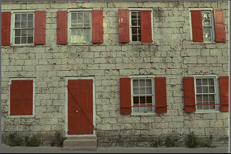
\includegraphics[width=1\textwidth]{24images/resize_kodim01.png}
\end{minipage}
\begin{minipage}{0.075\textwidth}
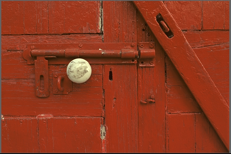
\includegraphics[width=1\textwidth]{24images/resize_kodim02.png}
\end{minipage}
\begin{minipage}{0.075\textwidth}
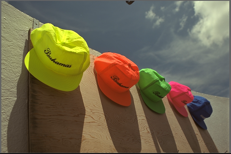
\includegraphics[width=1\textwidth]{24images/resize_kodim03.png}
\end{minipage}
\begin{minipage}{0.075\textwidth}
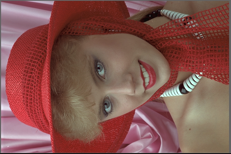
\includegraphics[width=1\textwidth]{24images/resize_kodim04.png}
\end{minipage}
\begin{minipage}{0.075\textwidth}
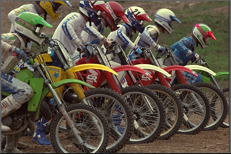
\includegraphics[width=1\textwidth]{24images/resize_kodim05.png}
\end{minipage}
\begin{minipage}{0.075\textwidth}
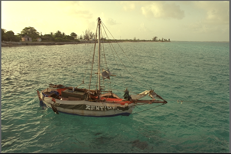
\includegraphics[width=1\textwidth]{24images/resize_kodim06.png}
\end{minipage}
}\vspace{-3mm}
\subfigure{
\begin{minipage}{0.075\textwidth}
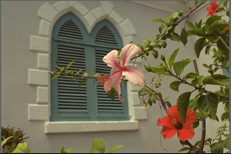
\includegraphics[width=1\textwidth]{24images/resize_kodim07.png}
\end{minipage}
\begin{minipage}{0.075\textwidth}
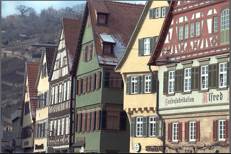
\includegraphics[width=1\textwidth]{24images/resize_kodim08.png}
\end{minipage}
\begin{minipage}{0.075\textwidth}
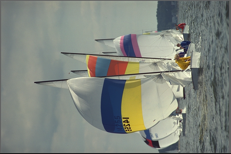
\includegraphics[width=1\textwidth]{24images/resize_kodim09.png}
\end{minipage}
\begin{minipage}{0.075\textwidth}
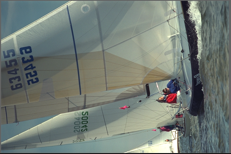
\includegraphics[width=1\textwidth]{24images/resize_kodim10.png}
\end{minipage}
\begin{minipage}{0.075\textwidth}
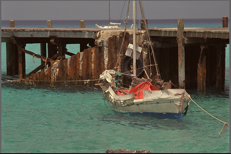
\includegraphics[width=1\textwidth]{24images/resize_kodim11.png}
\end{minipage}
\begin{minipage}{0.075\textwidth}
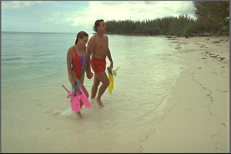
\includegraphics[width=1\textwidth]{24images/resize_kodim12.png}
\end{minipage}
}\vspace{-3mm}
\subfigure{
\begin{minipage}{0.075\textwidth}
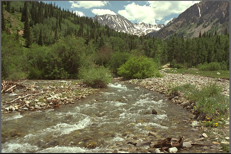
\includegraphics[width=1\textwidth]{24images/resize_kodim13.png}
\end{minipage}
\begin{minipage}{0.075\textwidth}
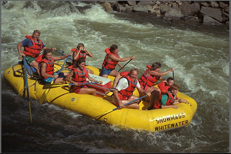
\includegraphics[width=1\textwidth]{24images/resize_kodim14.png}
\end{minipage}
\begin{minipage}{0.075\textwidth}
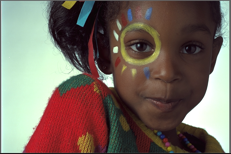
\includegraphics[width=1\textwidth]{24images/resize_kodim15.png}
\end{minipage}
\begin{minipage}{0.075\textwidth}
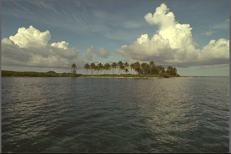
\includegraphics[width=1\textwidth]{24images/resize_kodim16.png}
\end{minipage}
\begin{minipage}{0.075\textwidth}
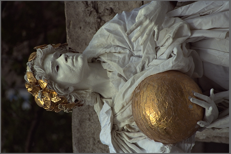
\includegraphics[width=1\textwidth]{24images/resize_kodim17.png}
\end{minipage}
\begin{minipage}{0.075\textwidth}
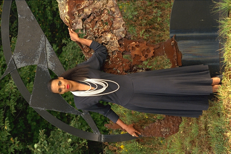
\includegraphics[width=1\textwidth]{24images/resize_kodim18.png}
\end{minipage}
}\vspace{-3mm}
\subfigure{
\begin{minipage}{0.075\textwidth}
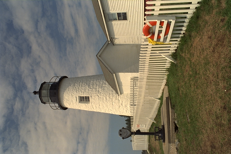
\includegraphics[width=1\textwidth]{24images/resize_kodim19.png}
\end{minipage}
\begin{minipage}{0.075\textwidth}
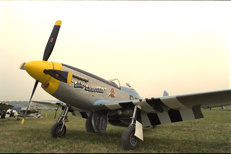
\includegraphics[width=1\textwidth]{24images/resize_kodim20.png}
\end{minipage}
\begin{minipage}{0.075\textwidth}
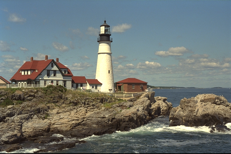
\includegraphics[width=1\textwidth]{24images/resize_kodim21.png}
\end{minipage}
\begin{minipage}{0.075\textwidth}
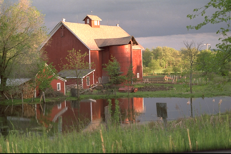
\includegraphics[width=1\textwidth]{24images/resize_kodim22.png}
\end{minipage}
\begin{minipage}{0.075\textwidth}
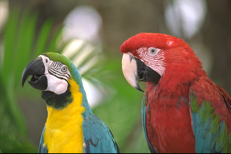
\includegraphics[width=1\textwidth]{24images/resize_kodim23.png}
\end{minipage}
\begin{minipage}{0.075\textwidth}
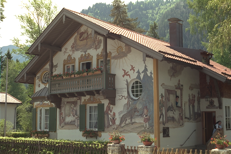
\includegraphics[width=1\textwidth]{24images/resize_kodim24.png}
\end{minipage}
}\vspace{-1mm}
\caption{The 24 high quality color images from the Kodak PhotoCD Dataset.}
\label{fig3}
\vspace{-2mm}
\end{figure}


\begin{table*}[t]
\caption{PSNR(dB) results of different denoising algorithms on 20 natural images.}
\label{tab1}
\begin{center}
\renewcommand\arraystretch{1.0}
\scriptsize
\begin{tabular}{|c||c|c|c|c|c|c|c|c|c|}
\hline
&\multicolumn{9}{c|}{ $\sigma_{r} = 40, \sigma_{g} = 20, \sigma_{b} = 30$}
\\
\hline
\hline
Image\#
&
\textbf{CBM3D}
&
\textbf{MLP}
&
\textbf{TNRD}
&
\textbf{Noise Clinic}
&
\textbf{Neat Image}
&
\textbf{WNNM}
&
\textbf{WNNMc}
&
\textbf{WNNMadmm}
&
\textbf{Multi-channel WNNM}
\\
\hline
1& 25.24 & 25.70 & 25.74 & 
\\
\hline
2& 28.27 & 30.12 & 30.21 & 
\\
\hline
3 & 28.81 & 31.19 & 31.49 & 
\\
\hline 
4 & 27.95 & 29.88 & 29.86 & 
\\
\hline
5 & 25.03 & 26.00 & 26.18 & 
\\
\hline
6 & 26.24 & 26.84 & 26.90 & 
\\
\hline
7 & 27.88 & 30.28 & 30.40 & 
\\
\hline
8 & 25.05 & 25.59 & 25.83 & 
\\
\hline
9 & 28.44 & 30.75 & 30.81 & 
\\
\hline
10 & 28.27 & 30.38 & 30.57 & 
\\
\hline
11 & 26.95 & 28.00 & 28.14 & 
\\
\hline
12 & 28.76 & 30.87 & 31.05 & 
\\
\hline
13 & 23.76 & 23.95 & 23.99 & 
\\
\hline
14 & 26.02 & 26.97 & 27.11 & 
\\
\hline
15 & 28.38 & 30.15 & 30.44 & 
\\
\hline
16 & 27.75 & 28.82 & 28.87 & 
\\
\hline
17 & 27.90 & 29.57 & 29.80 & 
\\
\hline
18 & 25.77 & 26.40 & 26.41 & 
\\
\hline
19 & 27.30 & 28.67 & 28.81 & 
\\
\hline
20 & 28.96 & 30.40 & 30.76 & 
\\
\hline
21 & 26.54 & 27.53 & 27.60 & 
\\
\hline
22 & 27.05 & 28.17 & 28.27 & 
\\
\hline
23 & 29.14 & 32.31 & 32.51 & 
\\
\hline
24 & 25.75 & 26.41 & 26.53 & 
\\
\hline
\textbf{Average} & 27.13 & 28.54 & 28.68 & 
\\
\hline
\end{tabular}
\end{center}
\end{table*}

\begin{figure*}\vspace{1mm}
\centering
\subfigure{
\begin{minipage}[t]{0.195\textwidth}
\centering
\raisebox{-0.15cm}{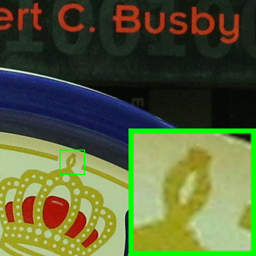
\includegraphics[width=1\textwidth]{images/resize_br_Noisy_5dmark3_iso3200_1_real.png}}
{\footnotesize (a) Noisy  \cite{crosschannel2016}: 37.00dB }
\end{minipage}
\begin{minipage}[t]{0.195\textwidth}
\centering
\raisebox{-0.15cm}{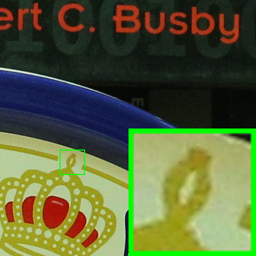
\includegraphics[width=1\textwidth]{images/resize_br_CBM3D_5dmark3_iso3200_1_real.png}}
{\footnotesize (b) CBM3D \cite{bm3d,cbm3d}: 37.02dB}
\end{minipage}
\begin{minipage}[t]{0.195\textwidth}
\centering
\raisebox{-0.15cm}{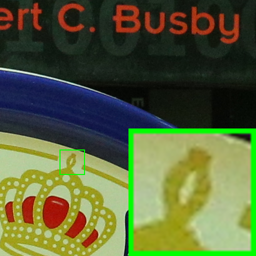
\includegraphics[width=1\textwidth]{images/resize_br_WNNM_5dmark3_iso3200_1_real.png}}
{\footnotesize (c) WNNM \cite{wnnm}: 37.01dB}
\end{minipage}
\begin{minipage}[t]{0.195\textwidth}
\centering
\raisebox{-0.15cm}{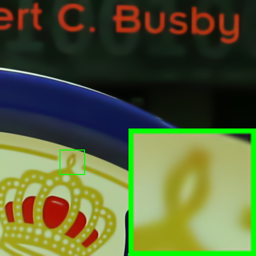
\includegraphics[width=1\textwidth]{images/resize_br_MLP_5dmark3_iso3200_1_real.png}}
{\footnotesize (d) MLP \cite{mlp}: 33.90dB }
\end{minipage}
\centering
\begin{minipage}[t]{0.195\textwidth}
\raisebox{-0.15cm}{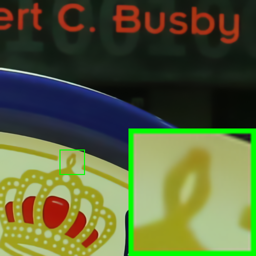
\includegraphics[width=1\textwidth]{images/resize_br_TRD_5dmark3_iso3200_1_real.png}}
{\footnotesize (e) TNRD \cite{chen2015learning}: 36.18dB  } 
\end{minipage}
}\vspace{-3mm}
\subfigure{
\begin{minipage}[t]{0.195\textwidth}
\centering
\raisebox{-0.15cm}{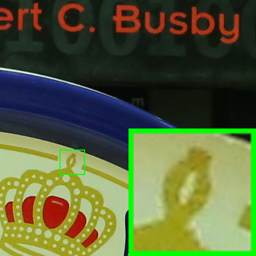
\includegraphics[width=1\textwidth]{images/resize_br_NI_5dmark3_iso3200_1_real.png}}
{\footnotesize (f) NI \cite{neatimage}: 37.68dB  }
\end{minipage}
\begin{minipage}[t]{0.195\textwidth}
\centering
\raisebox{-0.15cm}{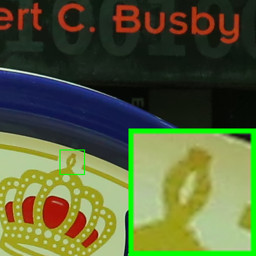
\includegraphics[width=1\textwidth]{images/resize_br_NC_5dmark3_iso3200_1_real.png}}
{\footnotesize (g) NC \cite{noiseclinic,ncwebsite}: 38.76dB  }
\end{minipage}
\begin{minipage}[t]{0.195\textwidth}
\centering
\raisebox{-0.15cm}{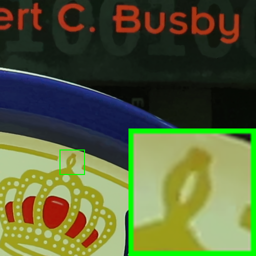
\includegraphics[width=1\textwidth]{images/resize_br_CCNoise_5dmark3_iso3200_1.png}}
{\footnotesize (h) CC \cite{crosschannel2016}: 38.37dB }
\end{minipage}
\begin{minipage}[t]{0.195\textwidth}
\centering
\raisebox{-0.15cm}{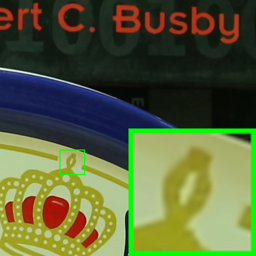
\includegraphics[width=1\textwidth]{images/resize_br_Guided_5dmark3_iso3200_1_real.png}}
{\footnotesize (i) Ours: \textbf{40.50}dB}
\end{minipage}
\begin{minipage}[t]{0.195\textwidth}
\centering
\raisebox{-0.15cm}{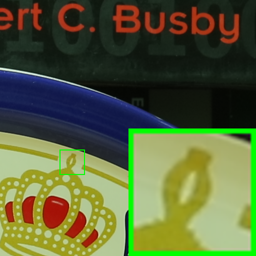
\includegraphics[width=1\textwidth]{images/resize_br_Mean_5dmark3_iso3200_1_real.png}}
{\footnotesize (j) Mean Image \cite{crosschannel2016}}
\end{minipage}
}\vspace{-0.5mm}
\caption{Denoised images of a region cropped from the real noisy image ``Canon 5D Mark 3 ISO 3200 1" \cite{crosschannel2016} by different methods. The images are better to be zoomed in on screen.}
\label{fig7}
\vspace{0.5mm}
\end{figure*}

\subsection{Experiments on Real Noisy Images}
In the second part, we compare the proposed method with other competing methods on the 15 real noisy images, , which are shown in Fig.\ 2, with ``ground truth'' clean images \cite{crosschannel2016}. The noisy images were collected under controlled indoor environment.\ Each scene was shot 500 times under the same camera and camera setting.\ The mean image of the 500 shots is roughly taken as the ``ground truth", with which the PSNR can be computed. Since the image size is very large (about $7000\times5000$) and the scenes of this dataset share repetitive contents, the authors of \cite{crosschannel2016} cropped 15 smaller images (of size $512\times512$) to perform experiments.

We firstly perform quantitative comparison on the 15 cropped images used in \cite{crosschannel2016}. The PSNR results of CBM3D \cite{bm3d}, WNNM \cite{wnnm}, MLP \cite{mlp}, CSF \cite{csf}, TNRD \cite{chen2015learning}, NC \cite{noiseclinic,ncwebsite}, NI \cite{neatimage} and
CC \cite{crosschannel2016} are listed in Table \ref{tab2} (The results of CC are copied from the original paper \cite{crosschannel2016}).\ The best and second best PSNR results of each image are highlighted in red and blue, respectively.\ One can see that on 9 out of the 15 images, our method achieves the best PSNR values.\ CC achieves the best PSNR on 3 of the 15 images.\ It should be noted that in the CC method, a specific model is trained for each camera and camera setting, while our method uses the same model for all images.\ On average, our proposed method has 0.28dB PSNR improvements over \cite{crosschannel2016} and much higher PSNR gains over other competing methods.\ Fig.\ \ref{fig7} shows the denoised images of a scene captured by Canon 5D Mark 3 at ISO = 3200.\ We can see that CBM3D, WNNM, NC, NI and CC would either remain noise or generate artifacts, while MLP, TNRD over-smooth much the image.\ By using the proposed multi-channel WNNM model, our method preserves the structures (e.g., edges and textures) better across the R, G, B channels and generate less artifacts than other denoising methods, leading to visually pleasant outputs.\ More visual comparisons can be found in the supplementary file.

\begin{figure}
\centering
\subfigure{
\begin{minipage}{0.085\textwidth}
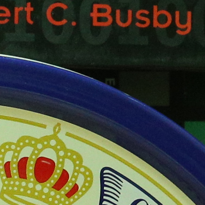
\includegraphics[width=1\textwidth]{CC15images/resize_5dmark3_iso3200_1_real.png}
\end{minipage}
\begin{minipage}{0.085\textwidth}
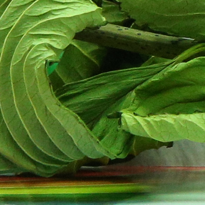
\includegraphics[width=1\textwidth]{CC15images/resize_5dmark3_iso3200_2_real.png}
\end{minipage}
\begin{minipage}{0.085\textwidth}
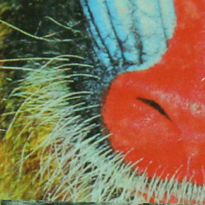
\includegraphics[width=1\textwidth]{CC15images/resize_5dmark3_iso3200_3_real.png}
\end{minipage}
\begin{minipage}{0.085\textwidth}
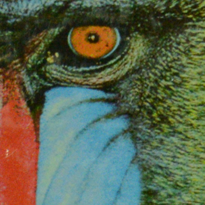
\includegraphics[width=1\textwidth]{CC15images/resize_d600_iso3200_1_real.png}
\end{minipage}
\begin{minipage}{0.085\textwidth}
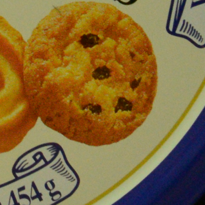
\includegraphics[width=1\textwidth]{CC15images/resize_d600_iso3200_2_real.png}
\end{minipage}
}\vspace{-3mm}
\subfigure{
\begin{minipage}{0.085\textwidth}
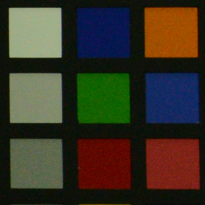
\includegraphics[width=1\textwidth]{CC15images/resize_d600_iso3200_3_real.png}
\end{minipage}
\begin{minipage}{0.085\textwidth}
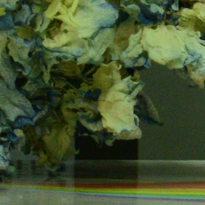
\includegraphics[width=1\textwidth]{CC15images/resize_d800_iso1600_1_real.png}
\end{minipage}
\begin{minipage}{0.085\textwidth}
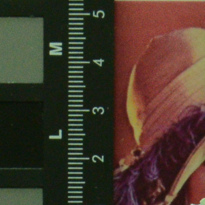
\includegraphics[width=1\textwidth]{CC15images/resize_d800_iso1600_2_real.png}
\end{minipage}
\begin{minipage}{0.085\textwidth}
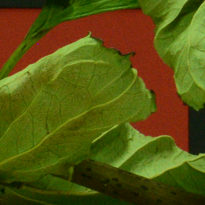
\includegraphics[width=1\textwidth]{CC15images/resize_d800_iso1600_3_real.png}
\end{minipage}
\begin{minipage}{0.085\textwidth}
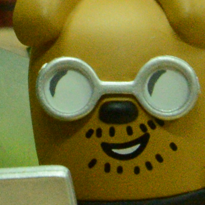
\includegraphics[width=1\textwidth]{CC15images/resize_d800_iso3200_1_real.png}
\end{minipage}
}\vspace{-3mm}
\subfigure{
\begin{minipage}{0.085\textwidth}
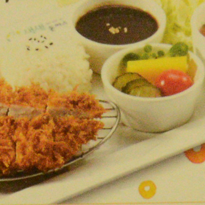
\includegraphics[width=1\textwidth]{CC15images/resize_d800_iso3200_2_real.png}
\end{minipage}
\begin{minipage}{0.085\textwidth}
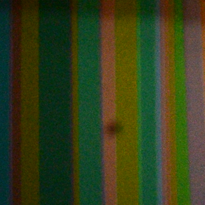
\includegraphics[width=1\textwidth]{CC15images/resize_d800_iso3200_3_real.png}
\end{minipage}
\begin{minipage}{0.085\textwidth}
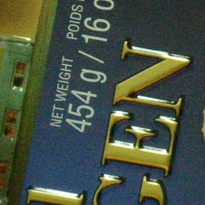
\includegraphics[width=1\textwidth]{CC15images/resize_d800_iso6400_1_real.png}
\end{minipage}
\begin{minipage}{0.085\textwidth}
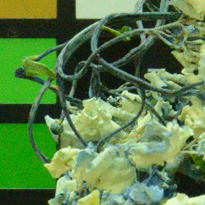
\includegraphics[width=1\textwidth]{CC15images/resize_d800_iso6400_2_real.png}
\end{minipage}
\begin{minipage}{0.085\textwidth}
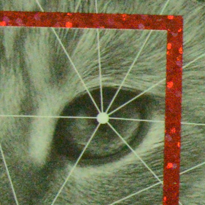
\includegraphics[width=1\textwidth]{CC15images/resize_d800_iso6400_3_real.png}
\end{minipage}
}\vspace{-1mm}
\caption{The 15 cropped real noisy images used in \cite{crosschannel2016}.}
\label{fig3}
\vspace{-2mm}
\end{figure}


\begin{table*}\vspace{2mm}
\caption{PSNR(dB) results of different methods on 15 cropped real noisy images used in \cite{crosschannel2016}.}
\vspace{0.5mm}
\label{tab2}
\begin{center}
\renewcommand\arraystretch{1}
\begin{tabular}{|c||c|c|c|c|c|c|c|c|c|c|}
\hline
Camera Settings & \textbf{Noisy} &\textbf{CBM3D}&\textbf{WNNM}&\textbf{MLP}&\textbf{CSF}&\textbf{TNRD}& \textbf{NI}& \textbf{NC}& \textbf{CC} &\textbf{Ours} 
\\
\hline
\multirow{3}{*}{\small{Canon 5D Mark III}} 
& 37.00 & 37.08 & 37.09 & 33.92 & 35.68 & 36.20 & 37.68 & {\color{blue}{38.76}} & 38.37 & {\color{red}{40.50}}
\\ 
\cdashline{2-11} 
\multirow{3}{*}{ISO = 3200}   
& 33.88 & 33.94 & 33.93 & 33.24 & 34.03 & 34.35 & 34.87 & {\color{blue}{35.69}} & 35.37 & {\color{red}{37.05}}
\\ 
\cdashline{2-11}    
& 33.83 & 33.88 & 33.90 & 32.37 & 32.63 & 33.10 & 34.77 & {\color{blue}{35.54}} & 34.91 & {\color{red}{36.11}}  
\\
\hline
\multirow{3}{*}{Nikon D600} 
& 33.28 & 33.33 & 33.34 & 31.93 & 31.78 & 32.28 & 34.12 & {\color{red}{35.57}} & {\color{blue}{34.98}} & 34.88
\\ 
\cdashline{2-11} 
\multirow{3}{*}{ISO = 3200}   
& 33.77 & 33.85 & 33.79 & 34.15 & 35.16 & 35.34 & 35.36 & {\color{red}{36.70}} & 35.95 & {\color{blue}{36.31}}
\\ 
\cdashline{2-11}    
& 34.93 & 35.02 & 34.95 & 37.89 & 39.98 & {\color{blue}{40.51}} & 38.68 & 39.28 & {\color{red}{41.15}} & 39.23
\\
\hline
\multirow{3}{*}{Nikon D800} 
& 35.47 & 35.54 & 35.57 & 33.77 & 34.84 & 35.09 & 37.34 & {\color{blue}{38.01}} & 37.99 & {\color{red}{38.40}}
\\ 
\cdashline{2-11} 
\multirow{3}{*}{ISO = 1600}   
& 35.71 & 35.79 & 35.77 & 35.89 & 38.42 & 38.65 & 38.57 & 39.05 & {\color{blue}{40.36}} & {\color{red}{40.92}}
\\ 
\cdashline{2-11}    
& 34.81 & 34.92 & 34.95 & 34.25 & 35.79 & 35.85 & 37.87 & 38.20 & {\color{blue}{38.30}} & {\color{red}{38.97}}
\\
\hline
\multirow{3}{*}{Nikon D800} 
& 33.26 & 33.34 & 33.31 & 37.42 & 38.36 & 38.56 & 36.95 & 38.07 & {\color{red}{39.01}} & {\color{blue}{38.66}}
\\ 
\cdashline{2-11} 
\multirow{3}{*}{ISO = 3200}   
& 32.89 & 32.95 & 32.96 & 34.88 & 35.53 & 35.76 & 35.09 & 35.72 & {\color{blue}{36.75}} & {\color{red}{37.07}}
\\ 
\cdashline{2-11}    
& 32.91 & 32.98 & 32.96 & 38.54 & {\color{blue}{40.05}} & {\color{red}{40.59}} & 36.91 & 36.76 & 39.06 & 38.52
\\ 
\hline
\multirow{3}{*}{Nikon D800} 
& 29.63 & 29.66 & 29.71 & 33.59 & 34.08 & {\color{blue}{34.25}} & 31.28 & 33.49 & {\color{red}{34.61}} & 33.76
\\ 
\cdashline{2-11} 
\multirow{3}{*}{ISO = 6400}   
& 29.97 & 30.01 & 29.98 & 31.55 & 32.13 & 32.38 & 31.38 & 32.79 & {\color{blue}{33.21}} & {\color{red}{33.43}}
\\ 
\cdashline{2-11}    
& 29.87 & 29.90 & 29.95 & 31.42 & 31.52 & 31.76 & 31.40 & 32.86 & {\color{blue}{33.22}} & {\color{red}{33.58}}
\\
\hline
Average & 33.41 & 33.48 & 33.48 & 34.32 & 35.33 & 35.65 & 35.49 & 36.43 & {\color{blue}{36.88}} & {\color{red}{ 37.16}}
\\
\hline
\end{tabular}
\end{center}
\vspace{1mm}
\end{table*}

\begin{figure*}\vspace{1mm}
\centering
\subfigure{
\begin{minipage}[t]{0.195\textwidth}
\centering
\raisebox{-0.15cm}{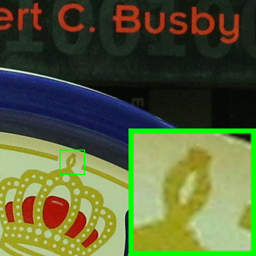
\includegraphics[width=1\textwidth]{images/resize_br_Noisy_5dmark3_iso3200_1_real.png}}
{\footnotesize (a) Noisy  \cite{crosschannel2016}: 37.00dB }
\end{minipage}
\begin{minipage}[t]{0.195\textwidth}
\centering
\raisebox{-0.15cm}{\includegraphics[width=1\textwidth]{images/resize_br_CBM3D_5dmark3_iso3200_1_real.png}}
{\footnotesize (b) CBM3D \cite{bm3d,cbm3d}: 37.02dB}
\end{minipage}
\begin{minipage}[t]{0.195\textwidth}
\centering
\raisebox{-0.15cm}{\includegraphics[width=1\textwidth]{images/resize_br_WNNM_5dmark3_iso3200_1_real.png}}
{\footnotesize (c) WNNM \cite{wnnm}: 37.01dB}
\end{minipage}
\begin{minipage}[t]{0.195\textwidth}
\centering
\raisebox{-0.15cm}{\includegraphics[width=1\textwidth]{images/resize_br_MLP_5dmark3_iso3200_1_real.png}}
{\footnotesize (d) MLP \cite{mlp}: 33.90dB }
\end{minipage}
\centering
\begin{minipage}[t]{0.195\textwidth}
\raisebox{-0.15cm}{\includegraphics[width=1\textwidth]{images/resize_br_TRD_5dmark3_iso3200_1_real.png}}
{\footnotesize (e) TNRD \cite{chen2015learning}: 36.18dB  } 
\end{minipage}
}\vspace{-3mm}
\subfigure{
\begin{minipage}[t]{0.195\textwidth}
\centering
\raisebox{-0.15cm}{\includegraphics[width=1\textwidth]{images/resize_br_NI_5dmark3_iso3200_1_real.png}}
{\footnotesize (f) NI \cite{neatimage}: 37.68dB  }
\end{minipage}
\begin{minipage}[t]{0.195\textwidth}
\centering
\raisebox{-0.15cm}{\includegraphics[width=1\textwidth]{images/resize_br_NC_5dmark3_iso3200_1_real.png}}
{\footnotesize (g) NC \cite{noiseclinic,ncwebsite}: 38.76dB  }
\end{minipage}
\begin{minipage}[t]{0.195\textwidth}
\centering
\raisebox{-0.15cm}{\includegraphics[width=1\textwidth]{images/resize_br_CCNoise_5dmark3_iso3200_1.png}}
{\footnotesize (h) CC \cite{crosschannel2016}: 38.37dB }
\end{minipage}
\begin{minipage}[t]{0.195\textwidth}
\centering
\raisebox{-0.15cm}{\includegraphics[width=1\textwidth]{images/resize_br_Guided_5dmark3_iso3200_1_real.png}}
{\footnotesize (i) Ours: \textbf{40.50}dB}
\end{minipage}
\begin{minipage}[t]{0.195\textwidth}
\centering
\raisebox{-0.15cm}{\includegraphics[width=1\textwidth]{images/resize_br_Mean_5dmark3_iso3200_1_real.png}}
{\footnotesize (j) Mean Image \cite{crosschannel2016}}
\end{minipage}
}\vspace{-0.5mm}
\caption{Denoised images of a region cropped from the real noisy image ``Canon 5D Mark 3 ISO 3200 1" \cite{crosschannel2016} by different methods. The images are better to be zoomed in on screen.}
\label{fig7}
\vspace{0.5mm}
\end{figure*}

\section{Conclusion}

The multiple channels in color images makes the color image denoising problem more interesting and challenging than grayscale image denoising. To explore the correlations among the R, G, B channels in color images, in this paper, we proposed a noval method for color image denoising. Specifically, we add a weighting matrix to the original weighted nuclear norm minimization model and break the property of having closed-form solution of the WNNM model. However, by adding a new variable and a linear constraint, we proposed to solve the new model via the ADMM algorithm. The problem can be solved in an alternative updating manner and both variables can be updated with closed-form solutions. The convergence results of the proposed algorithm, i.e., Algorithm 1, has also been proofed. The proposed multi-channel WNNM model has been applied in color image denoising including real noisy image denoising problem. Extensive experiments on benchmark datasets demonstrate the effectiveness of the proposed model. The introduce of the weighting matrix can indeed improve the performance of the WNNM method, which are designed for denoising grayscale images, for color image denoising. We believe this work can be extended in at least three directions. Firstly, the proposed weighting matrix can be introduced into other methods designed for denoising grayscale images. Secondly, the weighting matrix beyond the diagonal form, such as correlation form \cite{nearcor}, may bring better performance on color image denoising. Thirdly, the proposed multi-channel WNNM model can be further extended to deal with images with more channels, such as the hyperspectral images in remote sensing applications. We will focus our futhre work on these three directions.

\section{A. Proof of Theorem 1.}
\begin{proof}
1.\ Firstly, we proof that the sequence $\{\mathbf{A}_{k}\}$ generated by Algorithm 1 is upper bounded.
Let $\mathbf{X}_{k+1}+\rho_{k}^{-1}\mathbf{A}_{k}
=
\mathbf{U}_{k}\mathbf{\Sigma}_{k}\mathbf{V}_{k}^{\top}$
be its SVD in the $(k+1)$-th iteration. According to Corollary 1 of \cite{wnnmijcv}, we can have the SVD of $\mathbf{Z}_{k+1}$ as $\mathbf{Z}_{k+1}=\mathbf{U}_{k}\hat{\mathbf{\Sigma}}_{k}\mathbf{V}_{k}^{\top}=\mathbf{U}_{k}\mathcal{S}_{\frac{\bm{w}}{\rho_{k}}}(\mathbf{\Sigma}_{k})\mathbf{V}_{k}^{\top}$. 
Then we have 
\begin{align}
\|
\mathbf{A}_{k+1}
\|_{F}
&
=
\|
\mathbf{A}_{k}
+
\rho_{k}
(\mathbf{X}_{k+1}-\mathbf{Z}_{k+1})
\|_{F}
\\
&
=
\rho_{k}\|
\rho_{k}^{-1}
\mathbf{A}_{k}
+
\mathbf{X}_{k+1}
-
\mathbf{Z}_{k+1}
\|_{F}
\\
&
=
\rho_{k}\|
\mathbf{U}_{k}\mathbf{\Sigma}_{k}\mathbf{V}_{k}^{\top}
-
\mathbf{U}_{k}\mathcal{S}_{\frac{\bm{w}}{\rho_{k}}}(\mathbf{\Sigma}_{k})\mathbf{V}_{k}^{\top}
\|_{F}
\\
&
=
\rho_{k}\|
\mathbf{\Sigma}_{k}
-
\mathcal{S}_{\frac{\bm{w}}{\rho_{k}}}(\mathbf{\Sigma}_{k})
\|_{F}
\\
&
=
\rho_{k}
\sqrt{\sum_{i}(\mathbf{\Sigma}_{k}^{ii}-\mathcal{S}_{\frac{w_{i}}{\rho_{k}}}(\mathbf{\Sigma}_{k}^{ii}))^{2}}
\\
&
\le
\rho_{k}
\sqrt{\sum_{i}(\frac{w_{i}}{\rho_{k}})^{2}}
=
\sqrt{\sum_{i}w_{i}^{2}}.
\end{align}
The inequality above can be proofed as follows: given the diagonal matrix $\mathbf{\Sigma}_{k}$, we define $\mathbf{\Sigma}_{k}^{ii}$ as the $i$-th element of $\mathbf{\Sigma}_{k}^{ii}$. If $\mathbf{\Sigma}_{k}^{ii}\ge\frac{w_{i}}{\rho_{k}}$, we have $\mathcal{S}_{\frac{w_{i}}{\rho_{k}}}(\mathbf{\Sigma}_{k}^{ii})=\mathbf{\Sigma}_{k}^{ii}-\frac{w_{i}}{\rho_{k}}>0$. If $\mathbf{\Sigma}_{k}^{ii}<\frac{w_{i}}{\rho_{k}}$, we have $\mathcal{S}_{\frac{w_{i}}{\rho_{k}}}(\mathbf{\Sigma}_{k}^{ii})=0<\mathbf{\Sigma}_{k}^{ii}+\frac{w_{i}}{\rho_{k}}$. After all, we have $|\mathbf{\Sigma}_{k}^{ii}-\mathcal{S}_{\frac{w_{i}}{\rho_{k}}}(\mathbf{\Sigma}_{k}^{ii})|\le\frac{w_{i}}{\rho_{k}}$ and hence the inequality holds true. Hence, the sequence $\{\mathbf{A}_{k}\}$ is upper bounded.

2.\ Secondly, we proof that the sequence of Lagrangian function $\{\mathcal{L}(\mathbf{X}_{k+1},\mathbf{Z}_{k+1},\mathbf{A}_{k},\rho_{k})\}$ is also upper bounded. Since the global optimal solution of $\mathbf{X}$ and $\mathbf{Z}$ in corresponding subproblems, we always have 
$
\mathcal{L}(\mathbf{X}_{k+1},\mathbf{Z}_{k+1},\mathbf{A}_{k},\rho_{k})
\le
\mathcal{L}(\mathbf{X}_{k},\mathbf{Z}_{k},\mathbf{A}_{k},\rho_{k}).
$
Based on the updating rule that 
$
\mathbf{A}_{k+1}
=
\mathbf{A}_{k} + \rho_{k}(\mathbf{X}_{k+1}-\mathbf{Z}_{k+1})
$,
we have 
$
\mathcal{L}(\mathbf{X}_{k+1},\mathbf{Z}_{k+1},\mathbf{A}_{k+1},\rho_{k+1})
=
\mathcal{L}(\mathbf{X}_{k+1},\mathbf{Z}_{k+1},\mathbf{A}_{k},\rho_{k})
+
\langle
\mathbf{A}_{k+1}
-
\mathbf{A}_{k}
,
\mathbf{X}_{k+1}
-
\mathbf{Z}_{k+1}
\rangle
+
\frac{\rho_{k+1}-\rho_{k}}{2}
\|
\mathbf{X}_{k+1}-\mathbf{Z}_{k+1}
\|_{F}^{2}
=
\mathcal{L}(\mathbf{X}_{k+1},\mathbf{Z}_{k+1},\mathbf{A}_{k},\rho_{k})
+
\frac{\rho_{k+1}+\rho_{k}}{2\rho_{k}^{2}}
\|
\mathbf{A}_{k+1}
-
\mathbf{A}_{k}
\|_{F}^{2}
$.
Since the sequence 
$\{\|
\mathbf{A}_{k}\}$
is upper bounded, the sequence 
$\{\|
\mathbf{A}_{k+1}
-
\mathbf{A}_{k}
\|_{F}\}$ is also upper bounded. Denote by $a$ the upper bound of 
$\{\|
\mathbf{A}_{k+1}
-
\mathbf{A}_{k}
\|_{F}\}$, 
we have 
$
\mathcal{L}(\mathbf{X}_{k+1},\mathbf{Z}_{k+1},\mathbf{A}_{k+1},\rho_{k+1})
\le
\mathcal{L}(\mathbf{X}_{1},\mathbf{Z}_{1},\mathbf{A}_{0},\rho_{0})
+
a\sum_{k=0}^{\infty}\frac{\rho_{k+1}+\rho_{k}}{2\rho_{k}^{2}}
=
\mathcal{L}(\mathbf{X}_{1},\mathbf{Z}_{1},\mathbf{A}_{0},\rho_{0})
+
a\sum_{k=0}^{\infty}\frac{\mu+1}{2\mu^{k}\rho_{0}}
\le
\mathcal{L}(\mathbf{X}_{1},\mathbf{Z}_{1},\mathbf{A}_{0},\rho_{0})
+
\frac{a}{\rho_{0}}\sum_{k=0}^{\infty}\frac{1}{\mu^{k-1}}.
$
The last inequality holds since $\mu+1<2\mu$. Since $\sum_{k=0}^{\infty}\frac{1}{\mu^{k-1}}<\infty$, the sequence of Lagrangian function 
$\mathcal{L}(\mathbf{X}_{k+1},\mathbf{Z}_{k+1},\mathbf{A}_{k+1},\rho_{k+1})$
is upper bound.

3. Thirdly, we proof that the sequences of 
$\{\mathbf{X}_{k}\}$ and $\{\mathbf{Z}_{k}\}$ are upper bounded. Since 
$\|\mathbf{W}(\mathbf{Y}-\mathbf{X})\|_{F}^{2}
+
\|\mathbf{Z}\|_{\bm{w},*}
=
\mathcal{L}(\mathbf{X}_{k},\mathbf{Z}_{k},\mathbf{A}_{k-1},\rho_{k-1})
-
\langle
\mathbf{A}_{k},
\mathbf{X}_{k}-\mathbf{Z}_{k}
\rangle
-
\frac{\rho_{k}}{2}
\|
\mathbf{X}_{k}-\mathbf{Z}_{k}
\|_{F}^{2}
=
\mathcal{L}(\mathbf{X}_{k},\mathbf{Z}_{k},\mathbf{A}_{k-1},\rho_{k-1})
+
\frac{1}{2\rho_{k}}
(
\|
\mathbf{A}_{k-1}
\|_{F}^{2}
-
\|
\mathbf{A}_{k}
\|_{F}^{2}
)
$.
Thus $\{\mathbf{W}(\mathbf{Y}-\mathbf{X}_{k})\}$ and $\{\mathbf{Z}_{k}\}$ are upper bounded, and hence
the sequence $\{\mathbf{X}_{k}\}$ is bounded by Cauchy-Schwarz inequality and triangle inequality.
We can obtain that 
$
\lim_{k \to \infty} 
\|\mathbf{X}_{k+1}-\mathbf{Z}_{k+1}\|_{F}
=
\lim_{k \to \infty} 
\rho_{k}^{-1}
\|
\mathbf{A}_{k+1}
-
\mathbf{A}_{k}
\|_{F}
=
0
$ and the equation (1) is proofed.

4. Then we can proof that 
$
\lim_{k \to \infty} 
\|
\mathbf{X}_{k+1}
-
\mathbf{X}_{k}
\|_{F}
=
\lim_{k \to \infty} 
\|
(\mathbf{W}^{\top}\mathbf{W}
+
\frac{\rho_{k}}{2}
\mathbf{I})^{-1}
(\mathbf{W}^{\top}\mathbf{W}\mathbf{Y}
-
\mathbf{W}^{\top}\mathbf{W}\mathbf{Z}_{k}
-
\frac{1}{2}
\mathbf{A}_{k})
-
\rho_{k}^{-1}
(\mathbf{A}_{k}-\mathbf{A}_{k-1})
\|_{F}
\le
\lim_{k \to \infty} 
\|
(\mathbf{W}^{\top}\mathbf{W}
+
\frac{\rho_{k}}{2}
\mathbf{I})^{-1}
(\mathbf{W}^{\top}\mathbf{W}\mathbf{Y}
-
\mathbf{W}^{\top}\mathbf{W}\mathbf{Z}_{k}
-
\frac{1}{2}
\mathbf{A}_{k})
\|_{F}
+
\rho_{k}^{-1}\|
\mathbf{A}_{k}-\mathbf{A}_{k-1}
\|_{F}
=
0
$
and hence (2) is proofed. 

5. Then (3) can be proofed by checking that 
$
\lim_{k \to \infty} 
\|
\mathbf{Z}_{k+1}-\mathbf{Z}_{k}
\|_{F}
=
\lim_{k \to \infty} 
\|
\mathbf{X}_{k}+\rho_{k}^{-1}\mathbf{A}_{k-1}-\mathbf{Z}_{k}
+
\mathbf{X}_{k+1}-\mathbf{X}_{k}
+
\rho_{k}^{-1}
\mathbf{A}_{k-1}
+
\rho_{k}^{-1}
\mathbf{A}_{k}
-
\rho_{k}^{-1}
\mathbf{A}_{k+1}
\|_{F}
\le
\lim_{k \to \infty} 
\|
\mathbf{\Sigma}_{k-1}-\mathcal{S}_{\bm{w}/\rho_{k-1}}(\mathbf{\Sigma}_{k-1})
\|_{F}
+
\|
\mathbf{X}_{k+1}-\mathbf{X}_{k}
\|_{F}
+
\rho_{k}^{-1}
\|
\mathbf{A}_{k-1}
+
\mathbf{A}_{k+1}
-
\mathbf{A}_{k}
\|_{F}
=
0
$
,
where $\mathbf{U}_{k-1}\mathbf{\Sigma}_{k-1}\mathbf{V}_{k-1}^{\top}$ is the SVD of the matrix $\mathbf{X}_{k}+\rho_{k-1}\mathbf{A}_{k-1}$
.
\end{proof}


{
\small
\bibliographystyle{unsrt}
\bibliography{egbib}
}

\end{document}